% This paper is part of the single transits project.
% Copyright 2015 Dan Foreman-Mackey (NYU) and the co-authors listed below.
%
%  RULES OF THE GAME
%
%  * 80 characters
%  * line breaks at the ends of sentences
%  * eqnarrys ONLY
%  * ``light curve'' not ``light-curve'' or ``lightcurve''
%  * Do not put in any comments that might get tweeted by @OverheardOnAph
%    (or maybe do put in a few....)
%  * ``percent'' (not \%) is a unit, as is ppm, so 5~percent.
%  * that is all.
%

\documentclass[12pt,preprint]{aastex}

\pdfoutput=1

\usepackage{color,hyperref}
\definecolor{linkcolor}{rgb}{0,0,0.5}
\hypersetup{colorlinks=true,linkcolor=linkcolor,citecolor=linkcolor,
            filecolor=linkcolor,urlcolor=linkcolor}
\usepackage{url}
\usepackage{amssymb,amsmath}
\usepackage{subfigure}
\usepackage{booktabs}

\usepackage{natbib}
\bibliographystyle{apj}

\newcommand{\project}[1]{\textsl{#1}}
\newcommand{\kepler}{\project{Kepler}}
\newcommand{\KT}{\project{K2}}
\newcommand{\tess}{\project{TESS}}
\newcommand{\plato}{\project{PLATO}}
\newcommand{\jwst}{\project{JWST}}
\newcommand{\terra}{\project{TERRA}}
\newcommand{\pdc}{\project{PDC}}
\newcommand{\license}{MIT License}

\newcommand{\paper}{article}

\newcommand{\foreign}[1]{\emph{#1}}
\newcommand{\etal}{\foreign{et\,al.}}
\newcommand{\etc}{\foreign{etc.}}
\newcommand{\True}{\foreign{True}}
\newcommand{\Truth}{\foreign{Truth}}

\newcommand{\figref}[1]{\ref{fig:#1}}
\newcommand{\Fig}[1]{\figurename~\figref{#1}}
\newcommand{\fig}[1]{\Fig{#1}}
\newcommand{\figlabel}[1]{\label{fig:#1}}

\newcommand{\Tab}[1]{Table~\ref{tab:#1}}
\newcommand{\tab}[1]{\Tab{#1}}
\newcommand{\tablabel}[1]{\label{tab:#1}}

\renewcommand{\eqref}[1]{\ref{eq:#1}}
\newcommand{\Eq}[1]{Equation~(\eqref{#1})}
\newcommand{\eq}[1]{\Eq{#1}}
\newcommand{\eqalt}[1]{Equation~\eqref{#1}}
\newcommand{\eqlabel}[1]{\label{eq:#1}}

\newcommand{\sectionname}{Section}
\newcommand{\sectref}[1]{\ref{sect:#1}}
\newcommand{\Sect}[1]{\sectionname~\sectref{#1}}
\newcommand{\sect}[1]{\Sect{#1}}
\newcommand{\sectalt}[1]{\sectref{#1}}
\newcommand{\App}[1]{Appendix~\sectref{#1}}
\newcommand{\app}[1]{\App{#1}}
\newcommand{\sectlabel}[1]{\label{sect:#1}}

\newcommand{\T}{\ensuremath{\mathrm{T}}}
\newcommand{\dd}{\ensuremath{\,\mathrm{d}}}
\newcommand{\bvec}[1]{{\ensuremath{\boldsymbol{#1}}}}
\newcommand{\appropto}{\mathrel{\vcenter{
  \offinterlineskip\halign{\hfil$##$\cr
    \propto\cr\noalign{\kern2pt}\sim\cr\noalign{\kern-2pt}}}}}
\newcommand{\densityunit}{{\ensuremath{\mathrm{nat}^{-2}}}}

% TO DOS
\newcommand{\todo}[3]{{\color{#2}\emph{#1}: #3}}
\newcommand{\dfmtodo}[1]{\todo{DFM}{red}{#1}}
\newcommand{\hoggtodo}[1]{\todo{HOGG}{blue}{#1}}

% Notation for this paper.
\newcommand{\period}{{\ensuremath{P}}}
\newcommand{\rp}{{\ensuremath{R_\mathrm{P}}}}
\newcommand{\rate}{{\ensuremath{\Gamma}}}
\newcommand{\score}{{\ensuremath{S}}}

\newcommand{\datareleaseurl}{{\url{http://bbq.dfm.io/ketu}}}

% no more bad lines!
\sloppy\sloppypar

\begin{document}

\title{%
Automated detection \& characterization of long-period transits in the
\kepler\ archive
}

\newcommand{\uw}{3}
\newcommand{\nyu}{4}
\newcommand{\cds}{5}
\newcommand{\mpia}{6}
\newcommand{\mpis}{7}
\author{%
    Daniel~Foreman-Mackey\altaffilmark{1,2,\uw},
    David~W.~Hogg\altaffilmark{\nyu,\mpia,\cds},
    Bernhard~Sch\"olkopf\altaffilmark{\mpis},
    and others
}
\altaffiltext{1}         {To whom correspondence should be addressed:
                          \url{danfm@uw.edu}}
\altaffiltext{2}         {Sagan Fellow}
\altaffiltext{\uw}       {Astronomy Department, University of Washington,
                          Seattle, WA, 98195, USA}
\altaffiltext{\nyu}      {Center for Cosmology and Particle Physics,
                          Department of Physics, New York University,
                          4 Washington Place, New York, NY, 10003, USA}
\altaffiltext{\cds}      {Center for Data Science, New York University,
                          726 Broadway, 7th Floor, New York, NY, 10003, USA}
\altaffiltext{\mpia}     {Max-Planck-Institut f\"ur Astronomie,
                          K\"onigstuhl 17, D-69117 Heidelberg, Germany}
\altaffiltext{\mpis}     {Max Planck Institute for Intelligent Systems
                          Spemannstrasse 38, 72076 T\"ubingen, Germany}

\begin{abstract}

Hi.

\end{abstract}

\keywords{%
methods: data analysis
---
methods: statistical
---
catalogs
---
planetary systems
---
stars: statistics
}

\section{Introduction}

The transit method of exoplanet detection and characterization has been
demonstrated as a powerful method for building systematic catalogs of
exoplanets.
Despite the great success of the \kepler\ Mission with thousands of planet
discoveries \citep{Burke:2014, Rowe:2015}, current methods for exoplanet
discoveries are currently limited in the range of orbital periods that can be
studied.
Specifically, the standard transit search procedures only discover signals
with at least three observed transits \citep[for example][]{Petigura:2013,
Burke:2014, Rowe:2015}.
For \kepler, with a baseline of about four years, this sets an upper limit on
the detectable periods of just over a year.
In the Solar System, Jupiter---with a period of 12 years---dominates the
planetary dynamics and, since it would only exhibit at most one transit in the
\kepler\ data, it would be missed by most existing transit search procedures.
It is possible to discover long-period planets like this using targeted radial
velocity (RV) surveys \citep[for example][]{Butler:2006, Knutson:2014} but the
cost of implementing a systematic RV search is substantially higher than
searching the existing and forthcoming photometric data for single transits.

There are two main technical barriers to a search for single transit events.
The first is that the transit probability for long-period planets is very low;
scaling as $\propto\period^{-5/3}$ for orbital periods longer than the
baseline of contiguous observations.
Therefore, even if long-period planets are intrinsically common, they will
still be underrepresented in a transiting sample.
The second challenge is that there are substantial signals in the observed
light curves caused by stochastic processes---both instrumental
(pointing jitter, temperature variations, \etc) and astrophysical (stellar
variability, \etc)---that can masquerade as transit signals.
In practice, even using the most sophisticated systematics removal methods,
these false signal far outnumber the true single transits.

Nearly every transit search algorithm is built on the same principles and many
of the same decisions are made.
In particular, at the heart of most methods is a matched filtering step where
the likelihood of an approximate transit model is computed on a grid in the
physical parameters \citep[\kepler\ Data Processing
Handbook\footnote{\url{https://archive.stsci.edu/kepler/manuals/KSCI-19081-001_Data_Processing_Handbook.pdf}};][]{%
Petigura:2013, Huang:2013, Dressing:2015, Foreman-Mackey:2015}.
Using these methods, and substantial hand-curation, some long-period
transiting candidates have been published \citep[for example][]{Batalha:2013,
Huang:2013, Kipping:2014a}.
For more recent data releases, the community has settled on more conservative
selection criteria where candidates are required to have multiple transits
\citep[for example][]{Petigura:2013, Burke:2014, Rowe:2015}.
Even the \project{QATS} algorithm \citep{Carter:2013} for finding
quasiperiodic transits builds on much the same infrastructure.
This means that there has never been a systematic search for single transits
in the full \kepler\ dataset.

A qualitatively different approach to planet search is employed by the
\project{Planet Hunters} (PH)
project\footnote{\url{http://www.planethunters.org/}} \citep{Fischer:2012}.
PH is a ``citizen science'' project where visitors to the website look at
sections of light curve and mark the locations of transits that can be
identified visually.
Visual inspection can be a useful search technique for large single transits
because humans are able to robustly distinguish transit signals from the noise
and this project has yielded some promising long-period candidates and
confirmed planets \citep[for example][]{Wang:2013}.
One shortcoming of the PH method is that it can be difficult to fully quantify
the performance (completeness and reliability) of the search and PH does not
evaluate their users using synthetic transit signals as is now common practice
in the transit search literature.
This means that the PH sample of candidates cannot be used for robust
population inference.


\section{Data selection \& preparation}\sectlabel{data}

For the purposes of this \paper, we select the 40,000 brightest G and K dwarfs
from the \kepler\ catalog using the following parameters:

        % m = (4200 <= stlr.teff) & (stlr.teff <= 6100)
        % m &= stlr.radius <= 1.15
        % m &= stlr.dataspan > 365.25*2.
        % m &= stlr.dutycycle > 0.6
        % m &= stlr.rrmscdpp07p5 <= 1000.
        % m &= stlr.kepmag < 15.

\begin{itemize}
{\item $4200\unit{K} \le T_\mathfm{eff} \le 6100\unit{K}$}

\end{itemize}

We start with the PDC-MAP light curves downloaded from
MAST\footnote{\url{https://archive.stsci.edu/kepler/}}.



The \kepler\ Mission measured photometric time series for about 190,000 stars
at half-hour cadence for a baseline of over four years.
We aim to search these light curves for single transits of long-period planets
and single eclipses of binary stars.
These data are made available on
MAST\footnote{\url{https://archive.stsci.edu/kepler/}} and, for each target,
we downloaded the full set of long cadence light curve files provided by Data
Release 24 \citep{Thompson:2015}.
From these files, we extracted the PDC time series and split them into
``sections'' with no more than ten contiguous missing or flagged data points.
The PDC light curves have been corrected for the instrumental effects caused
by the spacecraft using a data-driven model of the focal plane
\citep{Stumpe:2012, Smith:2012}.
Crucially, an attempt is also made by the PDC procedure to remove sharp
instrumental artifacts like ``sudden pixel sensitivity dropouts (SPSDs)''.
The success rate of this correction procedure is much higher than in earlier
data releases but, as discussed in \sect{demo}, there remain some cases that
are not properly accounted for.

The goal of this project is to discover the transits of long-period planets
that have not yet been discovered.
Therefore, when studying the light curve of an eclipsing binary star or a star
with known transiting planet candidates---on shorter periods---we also remove
all the in-transit data for the candidate using the parameters provided by the
\project{NASA Exoplanet
Archive}\footnote{\url{http://exoplanetarchive.ipac.caltech.edu/}; We
downloaded the \texttt{cumulative} table of \kepler\ Objects of Interest on
2015-03-25.}.



\section{Candidate vetting}

\paragraph{Light curve}


\begin{figure}[p]
\begin{center}
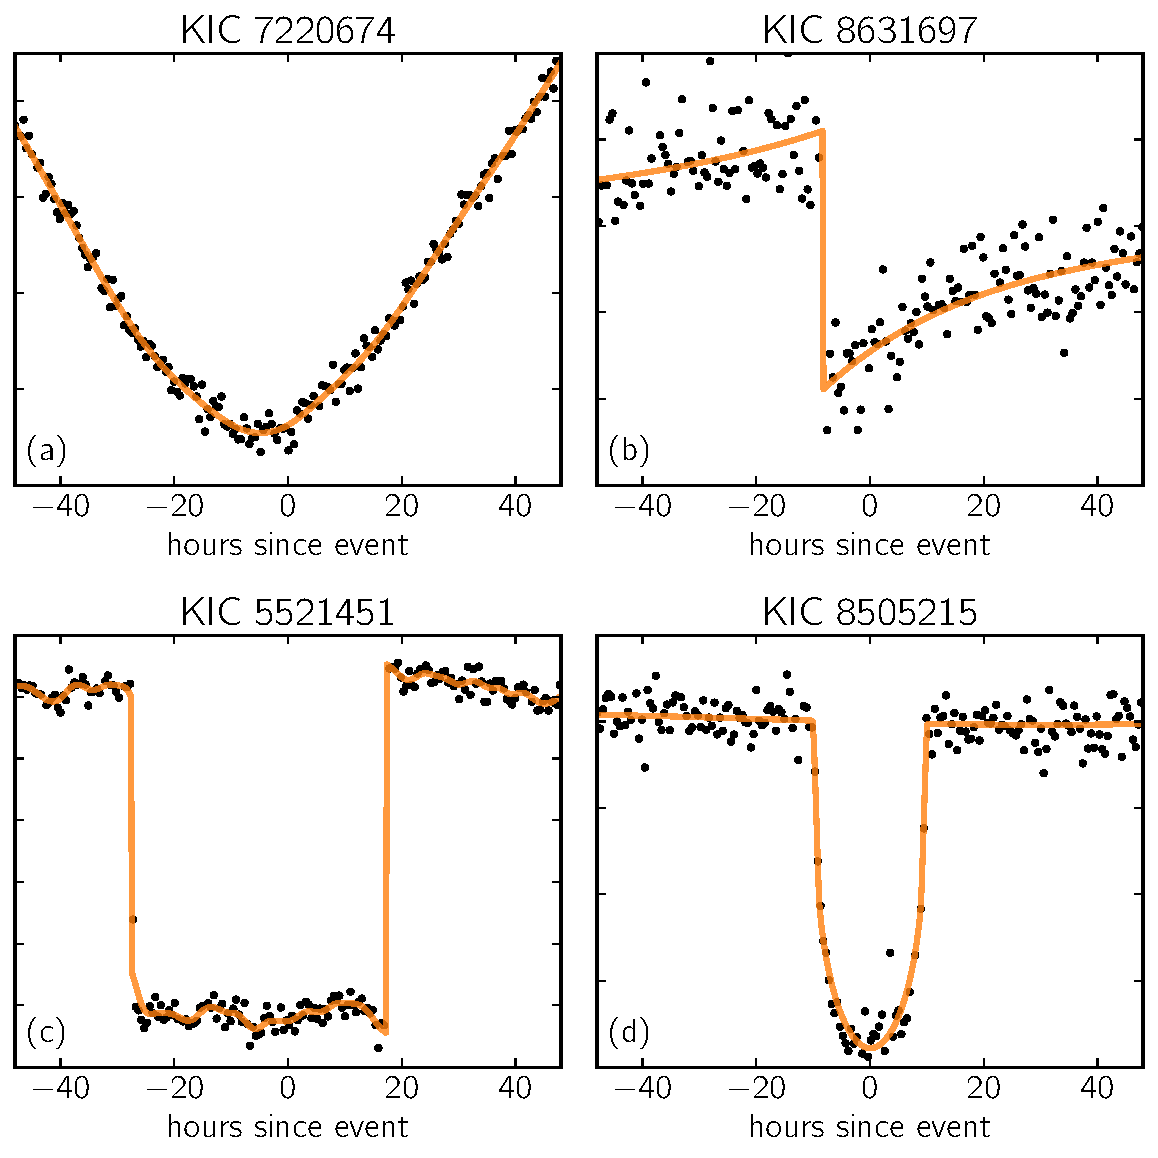
\includegraphics[width=\textwidth]{figures/model_comp.pdf}
\end{center}
\caption{%
Representative examples of candidate events flagged by the initial search.
Each example falls into a different model category and the figure shows the
data as black points and the best fit mean model prediction.
The examples represent the following model categories:
\emph{(a)} variability, \emph{(b)} step, \emph{(c)} box, and \emph{(d)}
transit.
\figlabel{model-comp}}
\end{figure}

\paragraph{Pixel-level}

Blah.

\paragraph{Auxiliary data}

Blah.


\section{Results}



\section{Completeness \& reliability}



\section{Discussion}\sectlabel{discussion}

The discovery and characterization of transiting planets based on a single
transit event is crucial for the future of transiting exoplanet surveys.
Many of the most dynamically influential planets---like Jupiter in our Solar
system---exhibit only a single transit in the full observational baseline of
the \kepler.
This will become even more of a problem as upcoming surveys move to shorter
contiguous observations.
For example, the \tess\ Mission is planned to get full-sky coverage at
half-hour cadence but most of the sky will only be targeted for a month.
This means that even habitable zone planets orbiting cool stars will transit
their host \emph{at most once in the entire lifetime of the Mission}!

To date, no methods exist for systematically and robustly discovering single
transit events based on large photometric surveys.
In this \paper, we present a novel and conceptually unique solution to this
problem drawing on machine learning methods for supervised classification.
This method has immense potential because it can be designed to be very robust
to false positives and it can exploit the detailed shape of physical transits.

Despite the fact that single transits are unlikely even if these long-period
planets are intrinsically common, we estimate that $\sim 60$ events should be
detectable in the \kepler\ archival dataset by extrapolating recent models of
planet occurrence rates and taking selection effects into account.
When applied to 3500 light curves from the \kepler\ dataset, this method
recovers one previously unknown single transit event at
$830.8093\pm0.0002$~KBJD in the light curve of KIC 10602068.
This rate is consistent with the predicted yield of 60 events in the full
dataset of 190,000 light curves.

Assuming a bound Keplerian orbit, we place constraints on the physical
properties of this transit candidate KIC 10602068.01.
Using photometrically derived stellar properties, we find that this candidate
has a radius of $2.1 \pm 0.4\,R_\mathrm{J}$ placing it as a very large planet
or brown dwarf or a small star.

This method for transit search is built using supervised classification and
its performance relies on several strong assumptions about the datasets and
these assumptions are sometimes violated leading to some transit-like signals
that appear to be caused by noise to be misclassified as transits.
The most severe assumption is that the noise properties of the data are
stationary.
In other words, we assume that variability in one subset of a light curve is
completely spanned by the variability in the other sections.
This assumption is, in general, false because the stochastic processes that
cause stellar variability are complicated and non-stationary and the detector
is plagued by non-negligible catastrophic changes in sensitivity and response.
We attempt to mitigate this problem by using light curves that have been
preprocessed to remove most of the instrumental effects and carefully dividing
the data into subsets but some false positives are still incorrectly
identified as candidates.

One possible method for reducing the false positive rate would be to augment
the training dataset using heuristic simulations of common false positives or
the light curves of ``similar'' stars.
Another option is to recognize that this search drastically reduces the
parameter space requiring evaluation and comparing the predictive power of
a transit model to other heuristic models including stellar variability or
instrumental effects.


\acknowledgments
It is a pleasure to thank
\ldots
for helpful contributions to the ideas and code presented here.
DFM and DWH were partially supported by the National Science Foundation
(grant IIS-1124794),
the National Aeronautics and Space Administration
(grant NNX12AI50G), and the Moore--Sloan Data Science Environment at NYU.

This research made use of the NASA \project{Astrophysics Data System} and the
NASA Exoplanet Archive.
The Archive is operated by the California Institute of Technology, under
contract with NASA under the Exoplanet Exploration Program.
This \paper\ includes data collected by the \kepler\ mission. Funding for the
\kepler\ mission is provided by the NASA Science Mission directorate.
We are grateful to the entire \kepler\ team, past and present.
Their tireless efforts were all essential to the tremendous success of the mission
and the successes of \KT, present and future.
These data were obtained from the Mikulski Archive for Space Telescopes
(MAST).
STScI is operated by the Association of Universities for Research in
Astronomy, Inc., under NASA contract NAS5-26555.
Support for MAST is provided by the NASA Office of Space Science via grant
NNX13AC07G and by other grants and contracts.

{\it Facilities:} \facility{Kepler}

\appendix

\section{Estimated yield}\sectlabel{est}

Before the launch of the \kepler\ Mission, \citet{Yee:2008} predicted the
yield of single transit events based on the planet occurrence rates estimated
based on small catalog of radial velocity discoveries \citep{Butler:2006} and
a fit to their occurrence rate \citep{Cumming:2008}.
Using these early results and the pre-launch specifications of the \kepler\
Mission, \citet{Yee:2008} predicted that \kepler\ would discover $\sim 6$
single transit events in the full dataset.
Now that the Mission is complete and we have better estimates of the
occurrence rate and distribution of planets \citep[for example][]{Dong:2013,
Petigura:2013, Foreman-Mackey:2014, Dressing:2015}, we can update the
predicted yield for single transit events in the \kepler\ light curves.
To make this estimate, we extrapolate the distribution of large planets on
relatively short orbits out to longer periods, taking detection efficiency
and the survey and targeting properties into account.

We will base our estimate on an assumed model $Q_k(\rp,\,\period)$ for the
absolute probability of detecting a planet with radius \rp\ and period
\period\ orbiting the star $k$, and the occurrence rate distribution
\begin{eqnarray}
\rate (\rp,\,\period) &=& \frac{\dd N}{\dd\ln\rp\dd\ln\period} \quad,
\end{eqnarray}
the expected number of planets per star, per logarithmic radius, per
logarithmic period.
Given these two quantities, the expected number of single transits in the
\kepler\ data is given by
\begin{eqnarray}
N &=& \sum_{k=1}^K N_k
\end{eqnarray}
where the sum is over the $K$ stars in the sample and $N_k$ is the expected
number of observable transits around star $k$
\begin{eqnarray}\eqlabel{nk}
N_k &=& \int Q_k(\rp,\,\period) \, \rate (\rp,\,\period)
    \dd\ln\rp \dd\ln\period \quad.
\end{eqnarray}
The integral in \eq{nk} is over the full range of target parameters.

For the purposes of this discussion, we assume an approximate simple detection
efficiency model with three contributions: the geometric transit probability,
the temporal transit probability, and signal-to-noise ratio threshold of the
search technique.
Assuming circular orbits, the geometric transit probability is given by
\citep{Winn:2010}
\begin{eqnarray}\eqlabel{q-geom}
Q_k^\mathrm{(geom)}(\rp,\,\period) &=& \frac{R_k}{a} \\
&=& \left( \frac{4\,\pi^2}{G\,M_k} \right)^{1/3} \, R_k \, \period^{-2/3}
\end{eqnarray}
where $R_k$ and $M_k$ are the radius and mass of the star $k$ respectively.
The eccentricity distribution of these long-period planets will affect this
transit probability \citep{Kipping:2014} but this simple prescription should
be sufficient for a rough estimate.
For long-period orbits, the temporal transit probability will be given by
\begin{eqnarray}\eqlabel{q-time}
Q_k^\mathrm{(time)}(\rp,\,\period) &=& \frac{T_k}{\period}
\end{eqnarray}
where $T_k$ is the total time that \kepler\ spent observing the star $k$.
Finally, the detection threshold depends on the detailed sensitivity of the
search procedure but we will approximate it as a simple step function in
signal-to-noise ratio of the transit.
This contribution will be given approximately by
\begin{eqnarray}
Q_k^\mathrm{(detect)}(\rp,\,\period) &=& \left\{\begin{array}{ll}
1 & \mathrm{if}\,\left(\rp/R_k\right)^2 > f\,\sigma_k \\
0 & \mathrm{otherwise}
\end{array}\right.
\end{eqnarray}
where $\sigma_k$ is an estimate of the noise in light curve of star $k$ and
$f$ is the detection threshold for the method.

Combining the detection efficiency components, the integral from \eq{nk}
becomes
\begin{eqnarray}\eqlabel{nk-2}
N_k &=& \left( \frac{4\,\pi^2}{G\,M_k} \right)^{1/3} \, R_k \, T_k
    \int_{\rp_\mathrm{min}} ^{\rp_\mathrm{max}} \frac{\dd\rp}{\rp}
    \int_{\period_\mathrm{min}} ^{\period_\mathrm{max}}
        \period^{-8/3}\,\rate(\rp,\,\period) \dd\period
\end{eqnarray}
where all the integration limits are set by the target parameter space.
Because of the detection probability threshold, $\rp_\mathrm{min}$ can be no
smaller than $R_k\,\sqrt{f\,\sigma_k}$.
\citet{Dong:2013} used the catalog of short period transiting planets found
by \kepler\ to constrain a model for the occurrence rate of large planets of
the form
\begin{eqnarray}
\rate(\rp,\,\period) &=& C\,\left(\frac{\period}{10\,\mathrm{d}}\right)^\beta
\end{eqnarray}
in a set of radius bins.
Using this model, the integral in \eq{nk-2} becomes
\begin{eqnarray}
N_k &=& \left( \frac{4\,\pi^2}{G\,M_k} \right)^{1/3} \, R_k \, T_k \,
    \sum_{j=1}^J \frac{C_j}{(10\,\mathrm{d})^{\beta_j}}\,
    \ln \left( \frac{\rp_{\mathrm{max},j}}{\rp_{\mathrm{min},j}} \right) \,
    \left[ \frac{{\period_\mathrm{min}}^{\beta_j - 5/3}}{5/3-\beta_j} \right]
\end{eqnarray}
where the sum is over the $J$ radial bins studied by \citet{Dong:2013}.
It's important to note that the model used by \citet{Dong:2013} is given in
base-10 logarithms so the units must be converted to natural logarithms as
appropriate.

Assuming the stellar parameters provided by the NASA Exoplanet
Archive\footnote{We downloaded the \texttt{q1\_q16\_stellar} table from
\url{http://exoplanetarchive.ipac.caltech.edu/} on 2015-04-03.}
\citep{Huber:2014} and approximating the stellar noise using the 15-hour CDPP
\citep{Christiansen:2012}, \fig{predict} shows the extrapolated number of
transiting planets with $1500\,\mathrm{d} < \period < 5000\,\mathrm{d}$ based
on the \citet{Dong:2013} power-law model.
For a detection threshold $f\sim10$, the expected number of single transit
events in the \kepler\ light curves is $\sim 60$.

This results is much more optimistic than the pre-launch estimate from
\citet{Yee:2008} for a few reasons.
One effect is that, the \kepler\ Mission ran for more than four
years---longer than the fiducial Mission goal---and $\sim190,000$ stars were
targeted for nearly the full baseline instead of the original 100,000.
\dfmtodo{Explain the other reasons.}


\clearpage
\bibliography{peerless}
\clearpage


% \begin{figure}[p]
% \begin{center}
% \includegraphics{figures/pca.pdf}
% \end{center}
% \caption{%
% The top 10 eigen light curves (ELCs) generated by running principal component
% analysis on all the aperture photometry from Campaign~1.
% \figlabel{pca}}
% \end{figure}

\end{document}
